Esta seção apresenta os procedimentos metodológicos utilizados para desenvolver e avaliar a abordagem proposta.  
O método, ilustrado na Figura~\ref{fig:method}, foi estruturado em quatro etapas principais: (i) materiais, (ii) pré-processamento, (iii) extração de características e treinamento do modelo, e (iv) avaliação de desempenho.  
Cada etapa é descrita em detalhes nas subseções a seguir.

\begin{figure}[H]
	\centering
	\makebox[\linewidth][l]{%
		\hspace*{-1cm}
		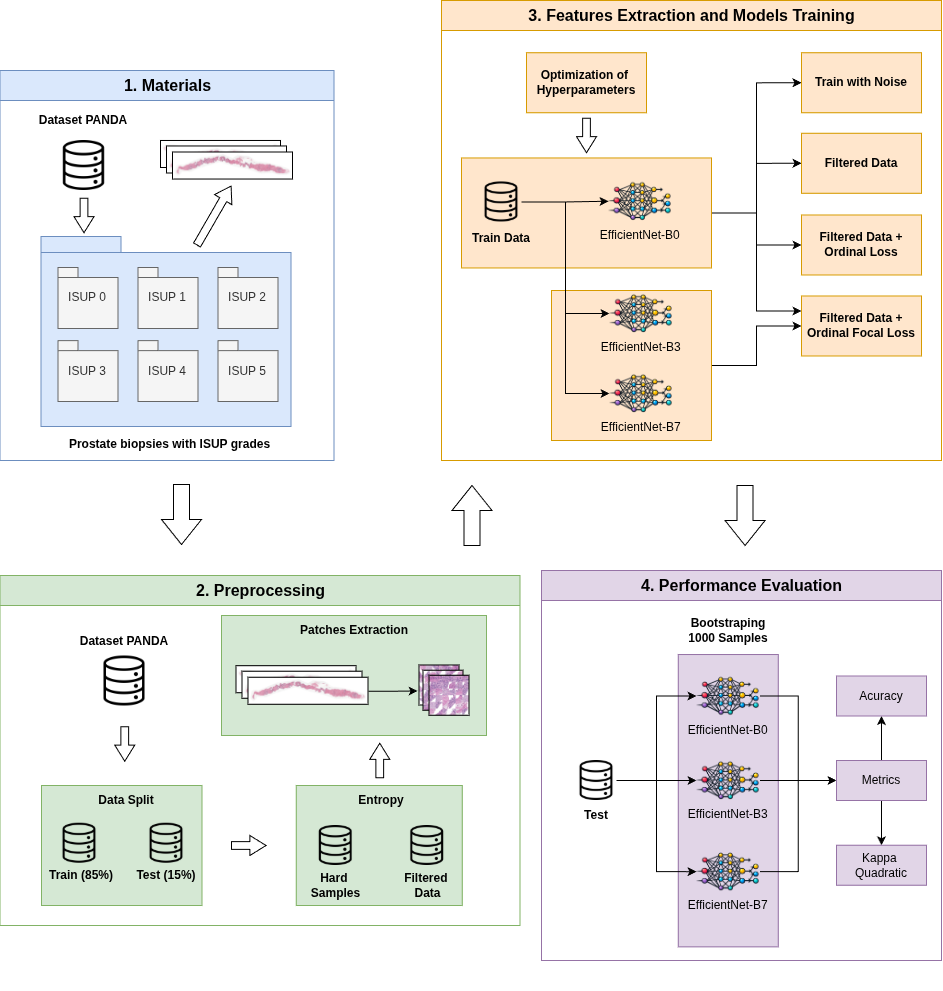
\includegraphics[width=1\linewidth]{images/method_bio.png}
	}
	
	\caption{Método proposto}
	\label{fig:method}
\end{figure}

\subsection{Materiais}
\label{sub:data}

Neste estudo, foi utilizado o conjunto de dados PANDA (\textit{Prostate Cancer Grade Assessment}), que consiste em aproximadamente 10.616 imagens histopatológicas de lâminas inteiras (WSIs) de biópsias de próstata \cite{ref-panda2020}.  
Esse conjunto foi disponibilizado como parte do desafio PANDA na plataforma Kaggle e tem sido amplamente utilizado em pesquisas sobre classificação automática do câncer de próstata.  

As imagens do dataset são anotadas com escores e graus de Gleason, fornecendo rótulos clínicos utilizados para a classificação da doença.  
Neste estudo, foi utilizada apenas a versão pública do dataset, sem acesso ao conjunto de teste privado disponibilizado durante o desafio.  

Os dados foram coletados de dois centros médicos, \textit{Radboud University Medical Center} e \textit{Karolinska Institute}, introduzindo variabilidade institucional nas imagens.  
Essa variabilidade está associada a diferenças nos protocolos de preparação das lâminas, nos procedimentos de digitalização e nos critérios de anotação, tornando o cenário experimental mais próximo da prática clínica real.  

Além disso, o dataset contém ruído inerente ao processo de aquisição e anotação das lâminas.  
Artefatos visuais incluem marcações de caneta feitas por patologistas durante a análise, conforme ilustrado na Figura~\ref{fig:pen_mask}.  
Também existem fontes de ruído relacionadas à rotulagem, como discordâncias entre anotadores na atribuição dos graus histopatológicos.  
Esses fatores aumentam a complexidade da tarefa de classificação automática e refletem desafios presentes na prática de patologia digital.

\begin{figure}[H]
	\centering
	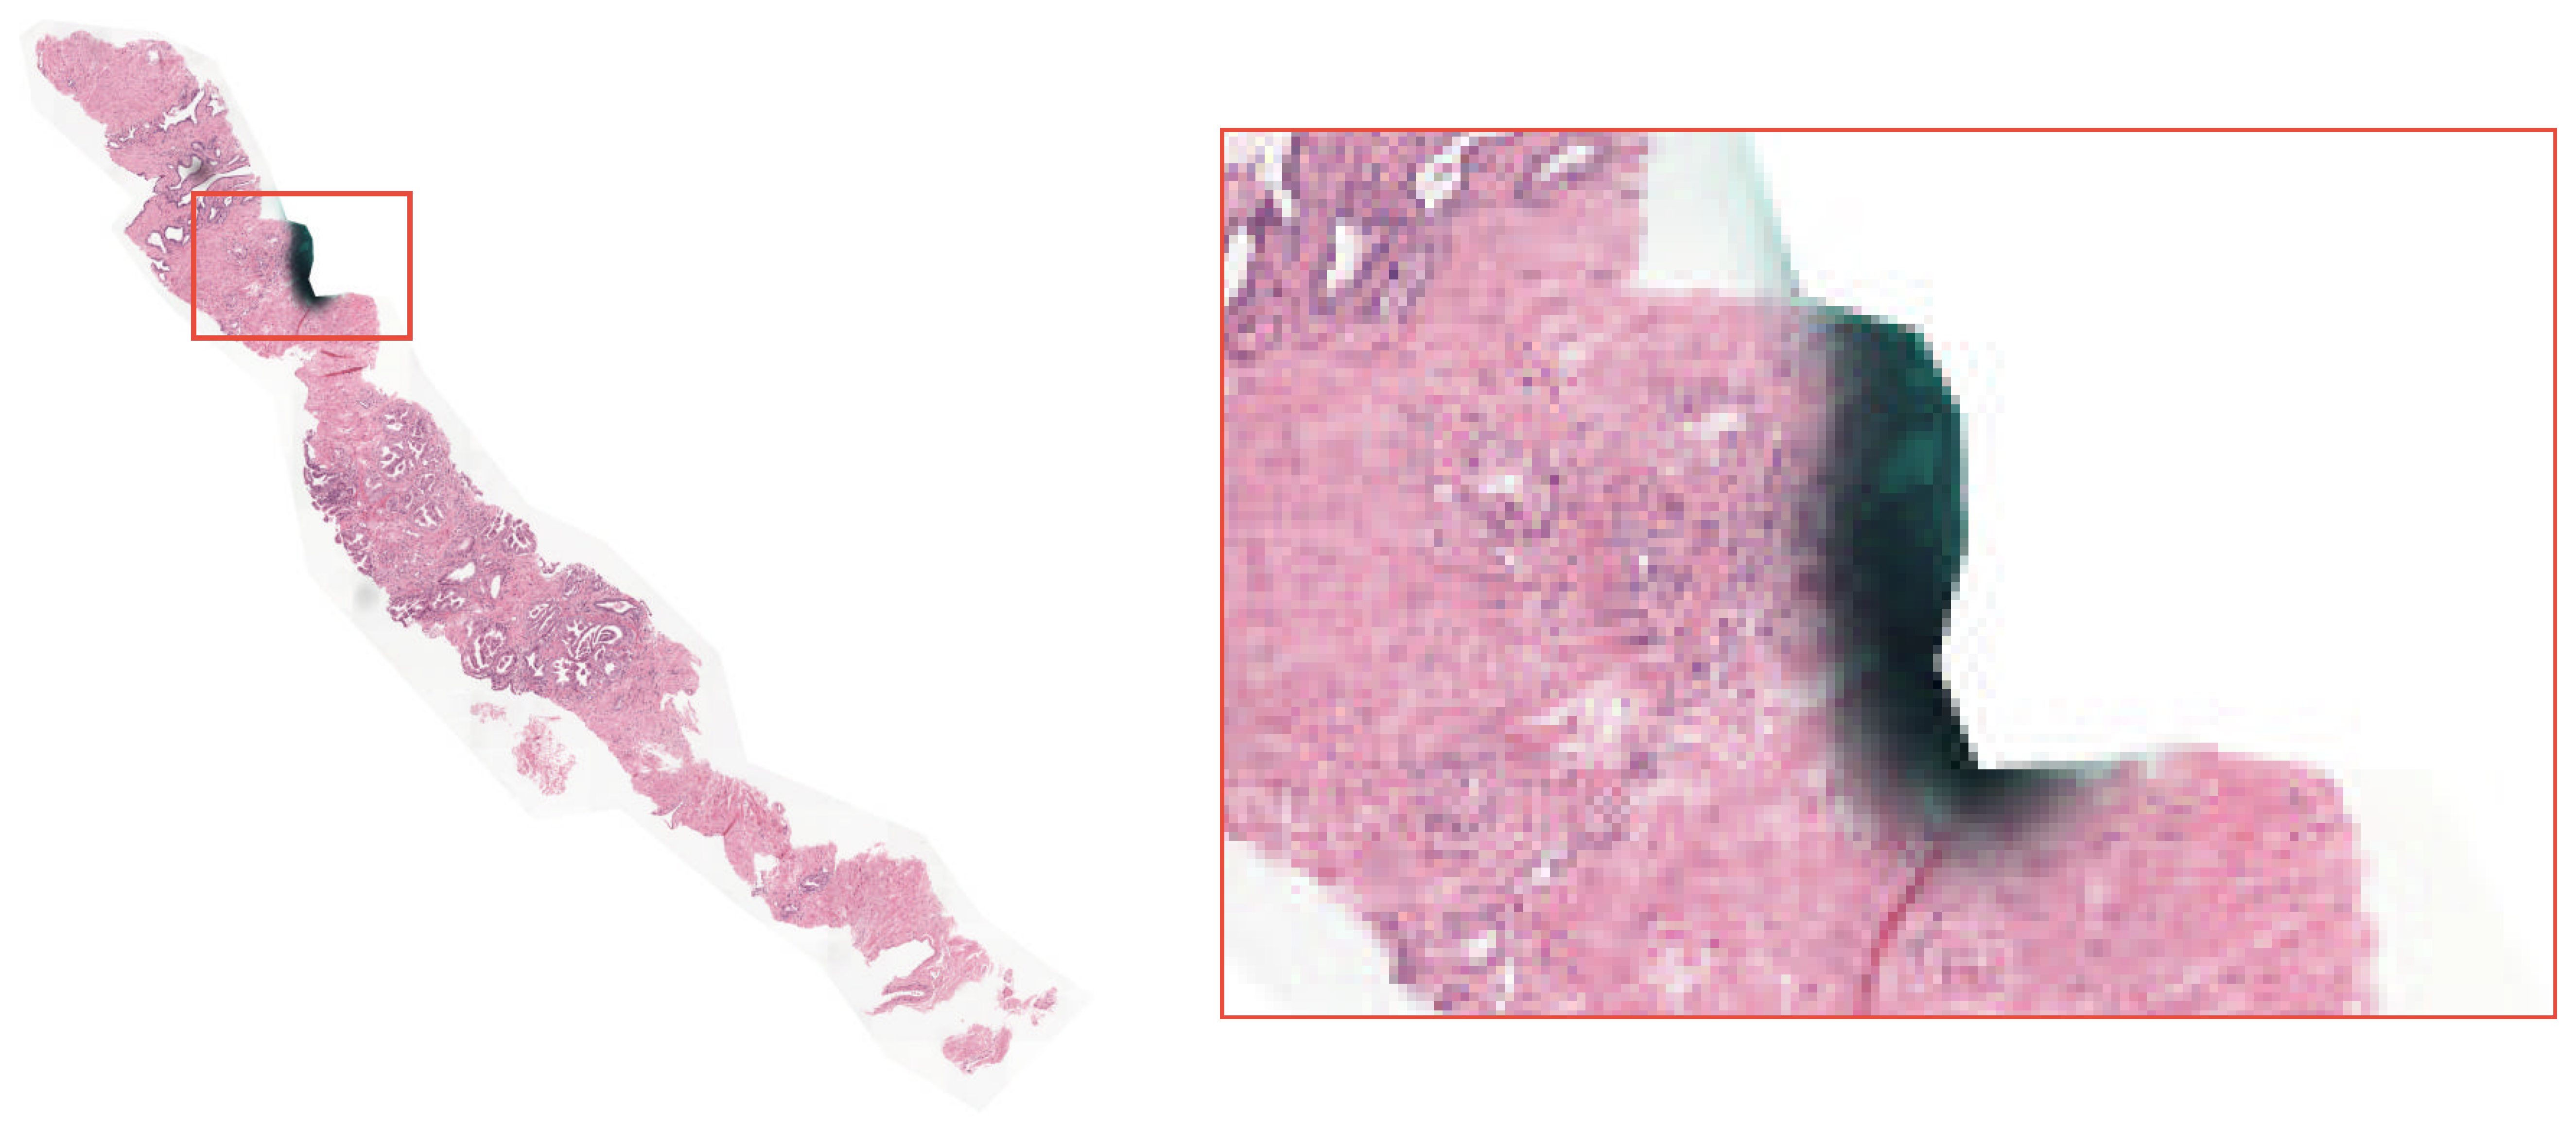
\includegraphics[width=0.8\linewidth]{images/zoom_region.png}
	\caption{Exemplo de artefato visual presente em uma WSI do dataset PANDA.  
		À esquerda, a lâmina completa com a região de interesse destacada em vermelho.  
		À direita, uma visualização ampliada revela uma marca de caneta sobre o tecido prostático.}
	\label{fig:pen_mask}
\end{figure}

Outro aspecto relevante do dataset é a distribuição desigual das amostras entre as seis classes de graduação (ISUP 0 a ISUP 5).  
Esse desbalanceamento é evidenciado na Tabela~\ref{fig:distribuicao-isup}, que apresenta a distribuição de amostras por classe.  
A maioria dos exemplos está concentrada nas classes ISUP 0 e ISUP 1.

\begin{figure}[htb]
	\centering
	\includegraphics[width=1\textwidth,height=0.3\textheight]{"images/distribuição_ISUP"}
	\caption{Distribuição de amostras no dataset PANDA}
	\label{fig:distribuicao-isup}	
\end{figure}

\subsection{Pré-processamento}
\label{sub:pre}

O fluxo de pré-processamento consistiu em duas etapas sequenciais: filtragem de ruído nos rótulos e extração de patches.  
Inicialmente, o dataset foi dividido em treino (85\%) e teste (15\%), garantindo independência entre o ajuste do modelo e a avaliação final.  
Após essa divisão, o conjunto de treino continha 9.024 instâncias, enquanto o conjunto de teste, utilizado para avaliação, possuía 1.592 instâncias.

\subsubsection{Filtragem de Ruído Baseada em Entropia}
\label{sub:entropia}

Conforme discutido na Seção~\ref{sub:data}, o dataset PANDA contém ruído de rótulos devido a anotações manuais e laudos inconclusivos. Para mitigar esse impacto, foi adotada uma estratégia baseada em incerteza preditiva.

Foram treinadas quatro variantes EfficientNet (B0, B1, B2 e B3), reservando 20\% do conjunto de treino para validação interna. Cada modelo gerou probabilidades para todas as amostras.

A incerteza foi quantificada usando entropia de Shannon:

\begin{equation}
	H = \frac{1}{C} \sum_{c=1}^{C} -[p_c\log(p_c) + (1-p_c)\log(1-p_c)]
\end{equation}

Amostras com maior entropia indicam maior incerteza.  
Os 10\% com maior entropia foram definidos como \textit{hard samples}.

\subsubsection{Extração de Patches}
\label{sub:patches}

Após a filtragem, foi realizada a geração de patches.  
Como mostrado na Figura~\ref{fig:original-panda}, grande parte da WSI é fundo branco.

\begin{figure}[H]
	\centering
	
\includegraphics[width=0.8\linewidth]{images/original.png}
	\caption{Exemplo de WSI com grande área sem tecido.}
	\label{fig:original-panda}
\end{figure}

Foi utilizado tamanho fixo de $256 \times 256$.  
Os patches foram ordenados por densidade de tecido e organizados em grades.

\begin{figure}[H]
	\centering
	
\includegraphics[width=0.9\textwidth]{images/tiles-original.png}	
	\caption{Extração de patches: 5$\times$5, 6$\times$6 e 7$\times$7.}
	\label{fig:tiles-original}
\end{figure}

A configuração 6$\times$6 foi escolhida como melhor compromisso.

\subsection{Extração de Características e Treinamento}

A EfficientNet-B0 foi usada como modelo base.  
Posteriormente, B3 e B7 foram avaliadas.

O problema foi reformulado como regressão ordinal.

Para um grau $k$, o rótulo é codificado como vetor cumulativo:  
exemplo: classe 3 $\rightarrow [1,1,1,0,0]$.

A função de perda combina \textit{focal loss}:

\[
\mathcal{L}_{focal} = - \frac{1}{K} \sum_{i=1}^{K}
\alpha_t (1 - p_t)^{\gamma} \log(p_t)
\]

com penalização ordinal:

\[
\hat{y} = \sum_{i=1}^{K} \hat{p}_i
\]

\[
|\hat{y} - y|
\]

Função final:

\[
\mathcal{L} = \lambda \cdot \mathcal{L}_{focal} + \beta \cdot |\hat{y} - y|
\]

\subsection{Avaliação de Desempenho}

A avaliação foi realizada com Accuracy e $\kappa_{\text{quad}}$.

Para análise estatística, foi aplicado bootstrap com 1.000 reamostragens, estimando média, desvio padrão e intervalo de confiança de 90\%.